In order to reduce power with a conventional receiver it has to be programmed to stay in sleeping mode until it is used again. However, it has to check whether any data was sent, therefore, it has to wake-up periodically to check if any notifications were sent. This duty cycle is a trade-off between power consumption and the respective response time. Conclusively, if the period between the notification checks is longer, the receiver is in an extended sleeping mode using less power, but simultaneously potentially missing out on a new notification, as the data can only be received in the running mode. The wakeup receiver now allows the device to be constantly in the listening mode, while consuming just a small amount of energy. Additionally to the system, the actual microcontroller, which coordinates the data transmission and other tasks stays shut down with only the wakeup receiver in listening mode. After receiving a defined pattern over this channel, the wakeup receiver generates an interrupt resulting in waking up the microcontroller. Subsequently, it establishes now a channel over a different wireless module, or execute another task. When finished, the microcontroller puts itself and all other modules (except the wakeup receiver) in sleep mode again. Figure \ref{theory:wake} shows a comparison of both the conventional approach and the solution with the wakeup receiver.
\begin{figure}[ht]
	\centering
	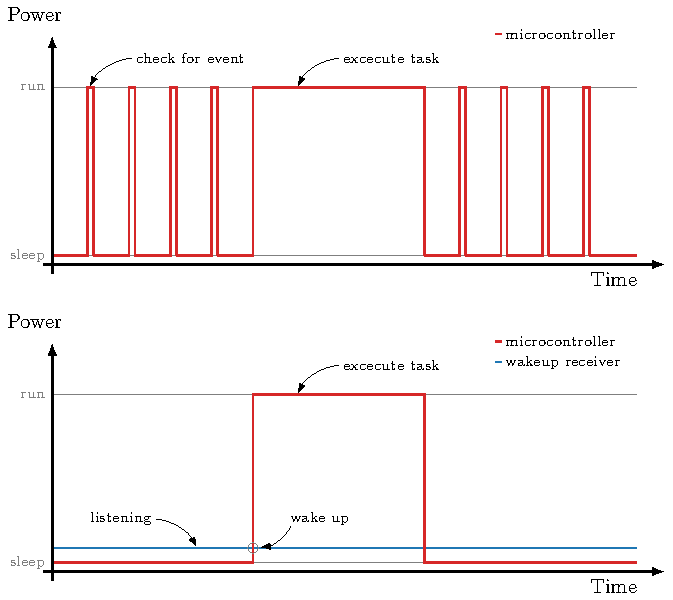
\includegraphics[width=0.9\textwidth]{2-theory/wakeup/graphics/wake_comp.pdf}
	\caption{Top: Microcontroller checks periodically for incoming data. Bottom: Constantly listening  wakeup receiver.\label{theory:wake}}
\end{figure}
One could argue, that the wakeup receiver module consumes in general more power, than the
microcontroller in sleep mode. However, since the microcontroller only wakes up when a task needs to be done, the overall energy consumption (area underneath the curve) is going to be smaller if the occurring wakeup event comes infrequently or over longer periods of time. The response time on the other hand can be kept in the microsecond range.
